\setcounter{section}{12}
\section{A Precise Full-Wave Rectifier: pt.I}

\subsection{Experiment Design}
    \subsubsection{Background}
        In the previous chapter, we constructed a half wave rectifier. However, the half wave rectifier has a low efficiency. In this chapter, we will construct a full wave rectifier to overcome these disadvantages. Here, we will construct one kind of percise full wave rectifier using two op-amps.

    \subsubsection{Propose}
    \begin{itemize}
        \item To verify one type precise full-wave rectifier
    \end{itemize}

\subsection{Experiment Design}
    \subsubsection{Materials}
        In this experiment, we will use the following components:
        \begin{itemize}
            \item 1N4148 Diode
            \item LM741 Op.Amp.
            \item Resistors
            \item Breadboard
            \item DC power supply
            \item Digital Multi-Meter
            \item Function Generator
            \item Oscilloscope
        \end{itemize}

    \subsubsection{Circuit Diagram}
        The following circuit diagrams 
        \begin{figure}[H]
            \centering
            \begin{subfigure}{0.6\textwidth}
                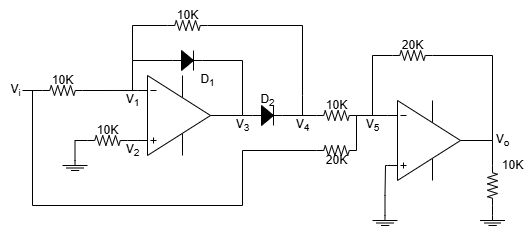
\includegraphics[width=1\linewidth]{Experiment_13/Circuit/Lab13.drawio.png}
                \caption{Full-Wave Rectifier Circuit I}
                \label{cir:13}
            \end{subfigure}
            \caption{}
        \end{figure}

    \subsubsection{Theoretical Analysis}
        \begin{enumerate}[a]
            \item \textbf{Inverting Amplifier}
        \end{enumerate}

\subsection{Experiment record}
    \subsubsection{AC Analysis}
    In the circuit shown in figure \ref{cir:13}, set the input signal frequency as 200Hz, and vary the amplitude, the output singal and the input signal is observed with the oscilloscope, and is shown in the following table.\par
    \begin{figure}[H]
        \centering
        \addtolength{\leftskip} {-2cm}
        \addtolength{\rightskip}{-2cm}

        \begin{subfigure}{0.3\linewidth}
            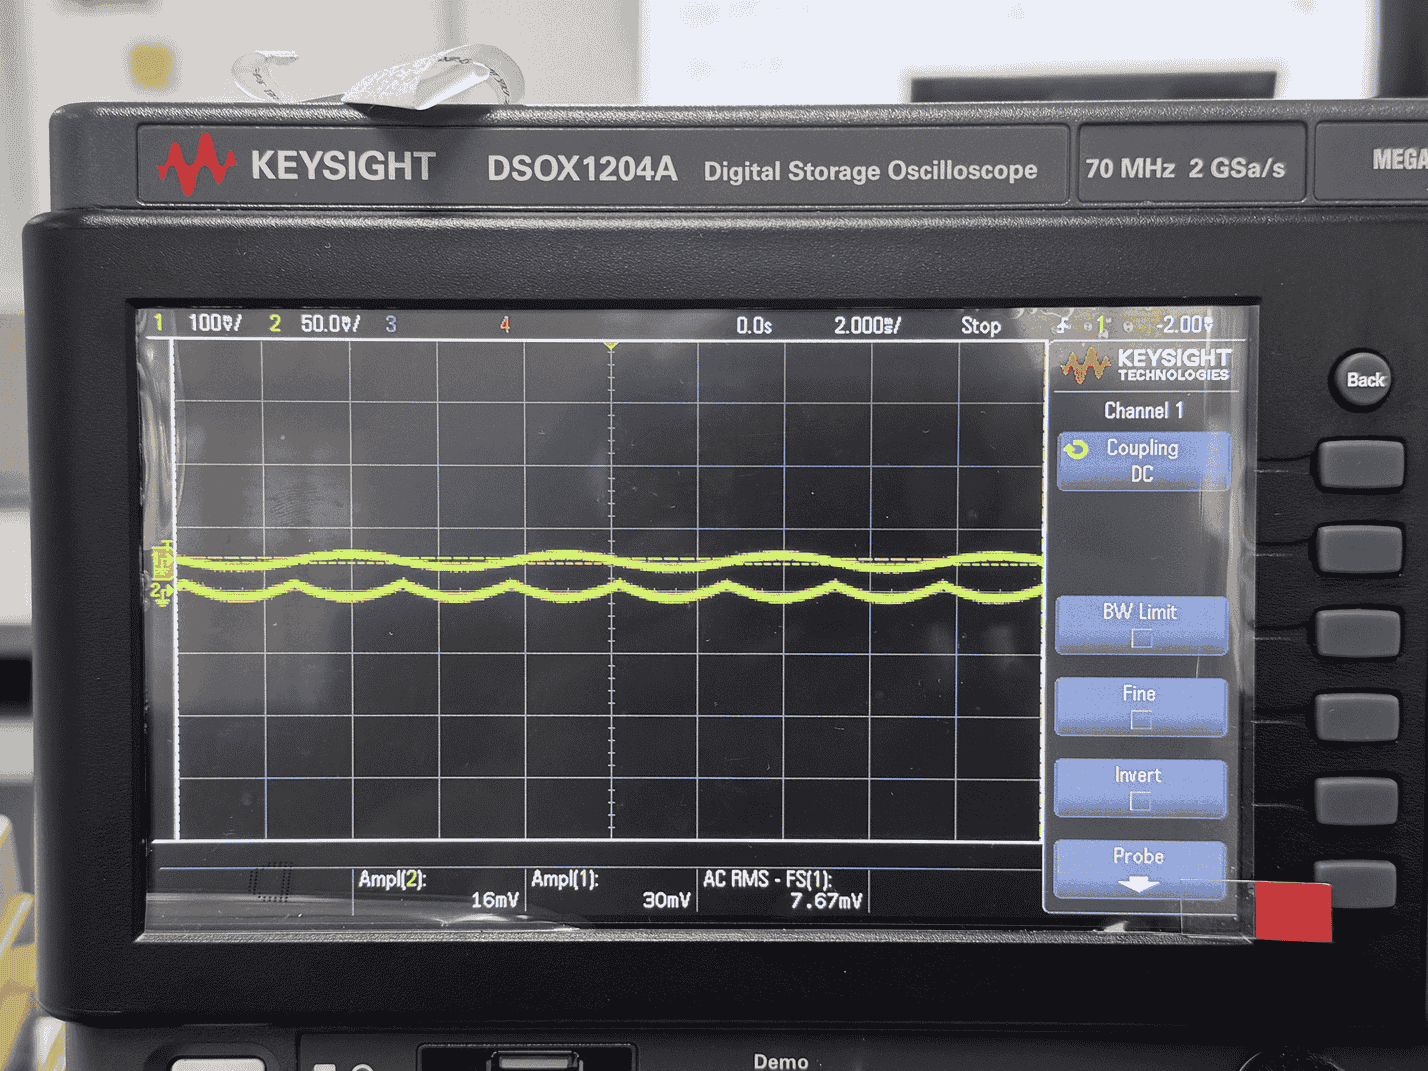
\includegraphics[width=1\linewidth]{Experiment_13/Images/13_0-1v.jpg}
            \caption{Amplitude $v_i=0.1V$}
            \label{wave:13-AC0}
        \end{subfigure}
        \begin{subfigure}{0.3\linewidth}
            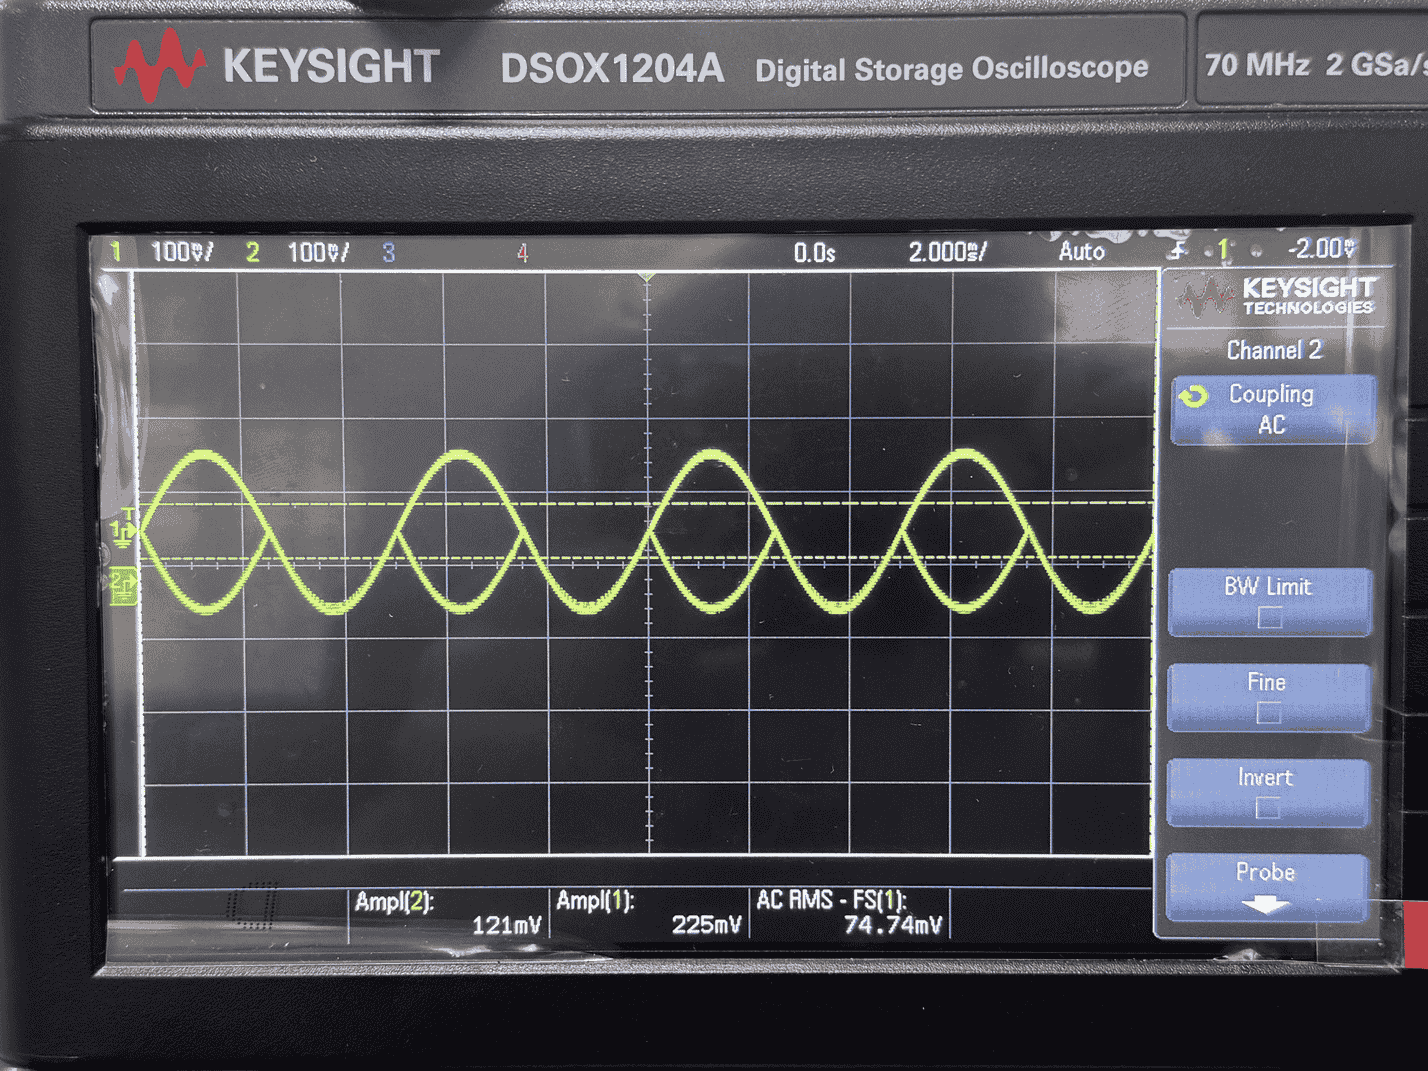
\includegraphics[width=1\linewidth]{Experiment_13/Images/13_1v.jpg}
            \caption{Amplitude $v_i=1V$}
            \label{wave:13-AC1}
        \end{subfigure}
        \begin{subfigure}{0.3\linewidth}
            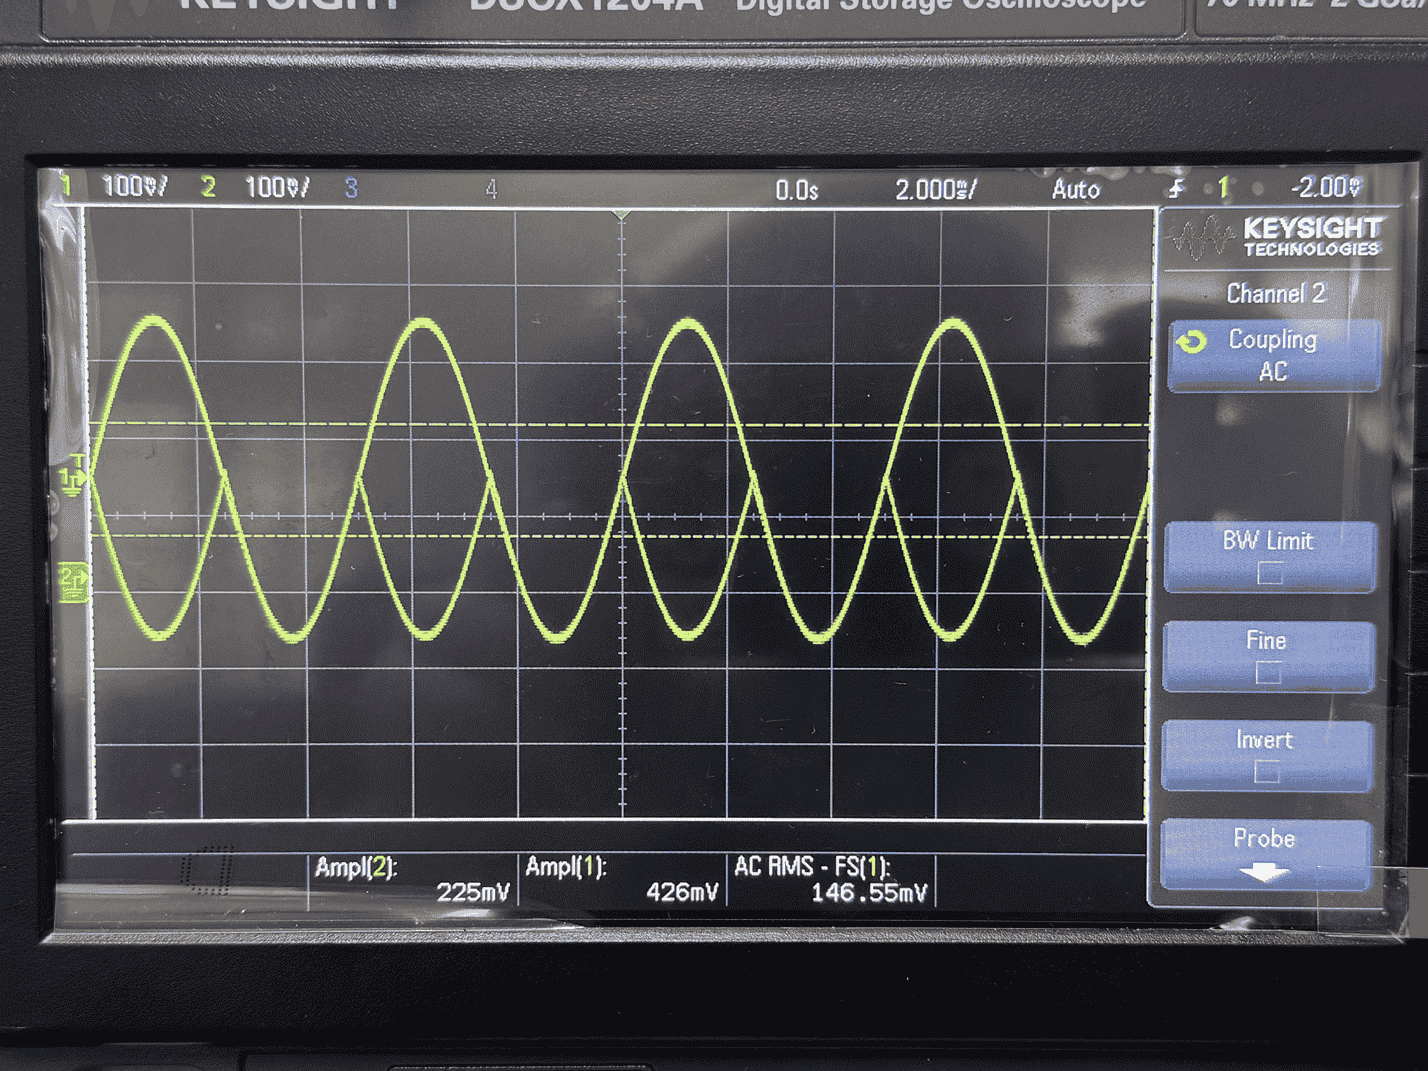
\includegraphics[width=1\linewidth]{Experiment_13/Images/13_2v.jpg}
            \caption{Amplitude $v_i=2V$}
            \label{wave:13-AC2}
        \end{subfigure}

        \begin{subfigure}{0.3\linewidth}
            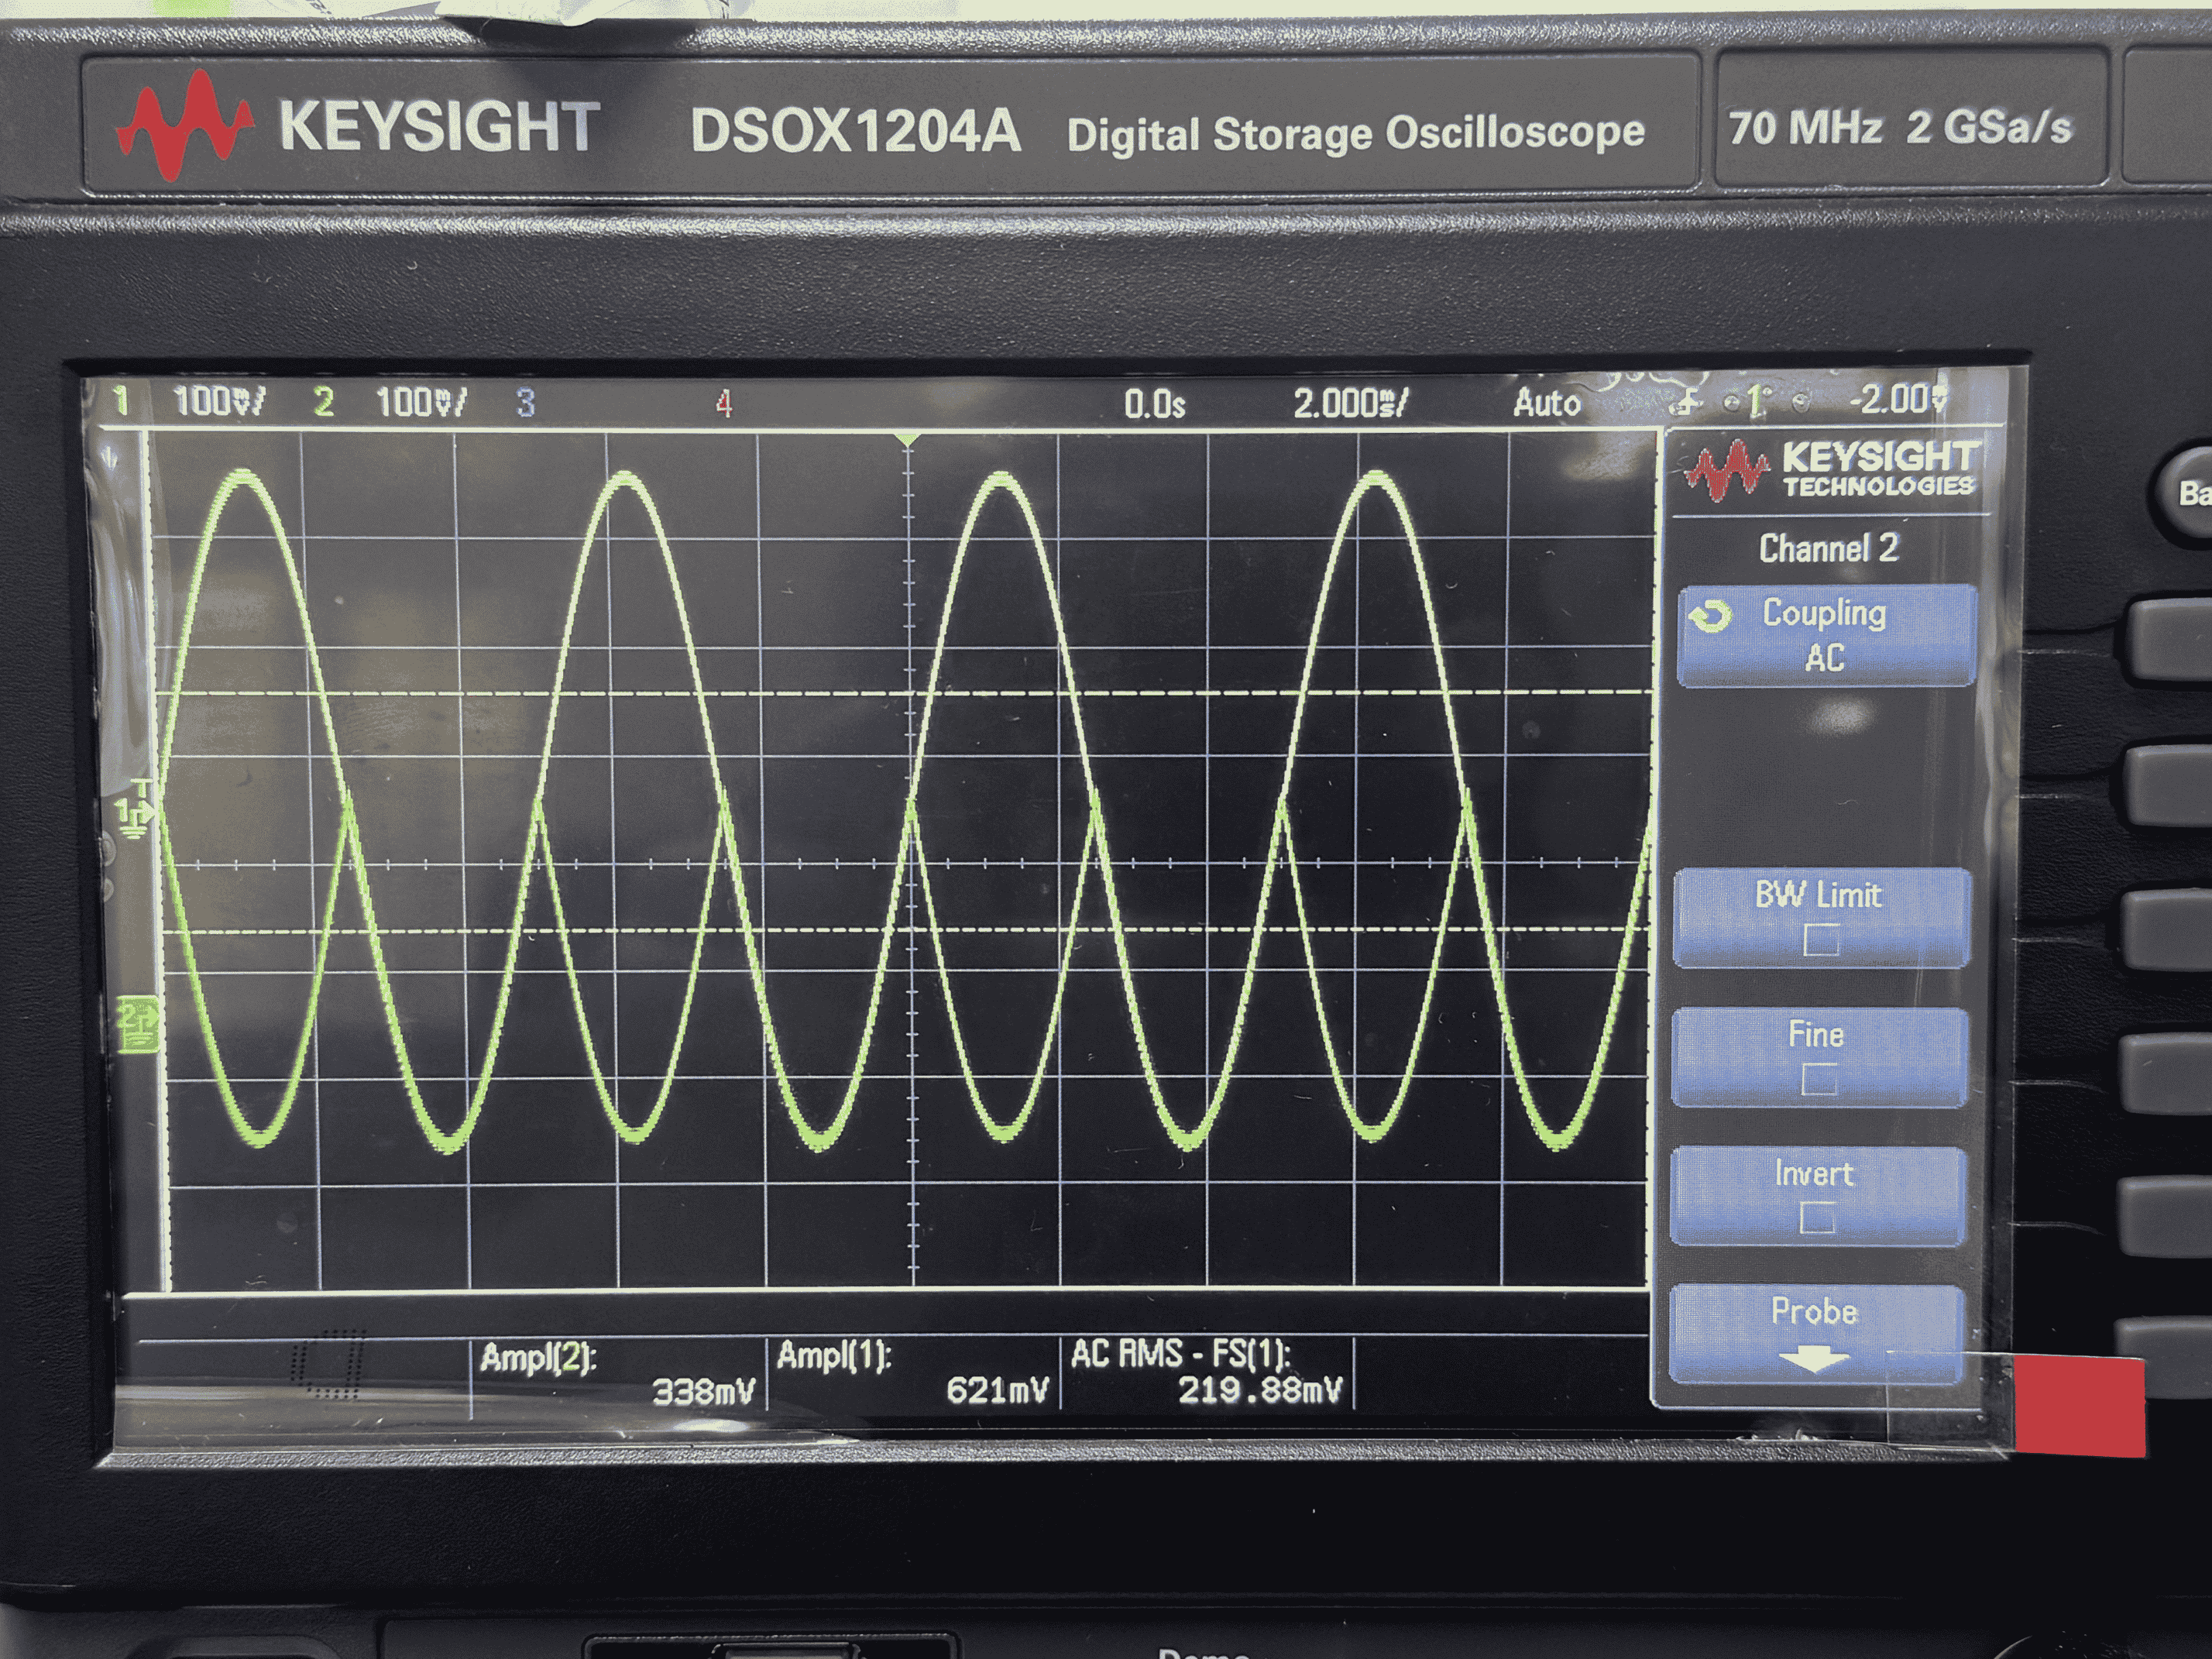
\includegraphics[width=1\linewidth]{Experiment_13/Images/13_3v.jpg}
            \caption{Amplitude $v_i=3V$}
            \label{wave:13-AC3}
        \end{subfigure}
        \begin{subfigure}{0.3\linewidth}
            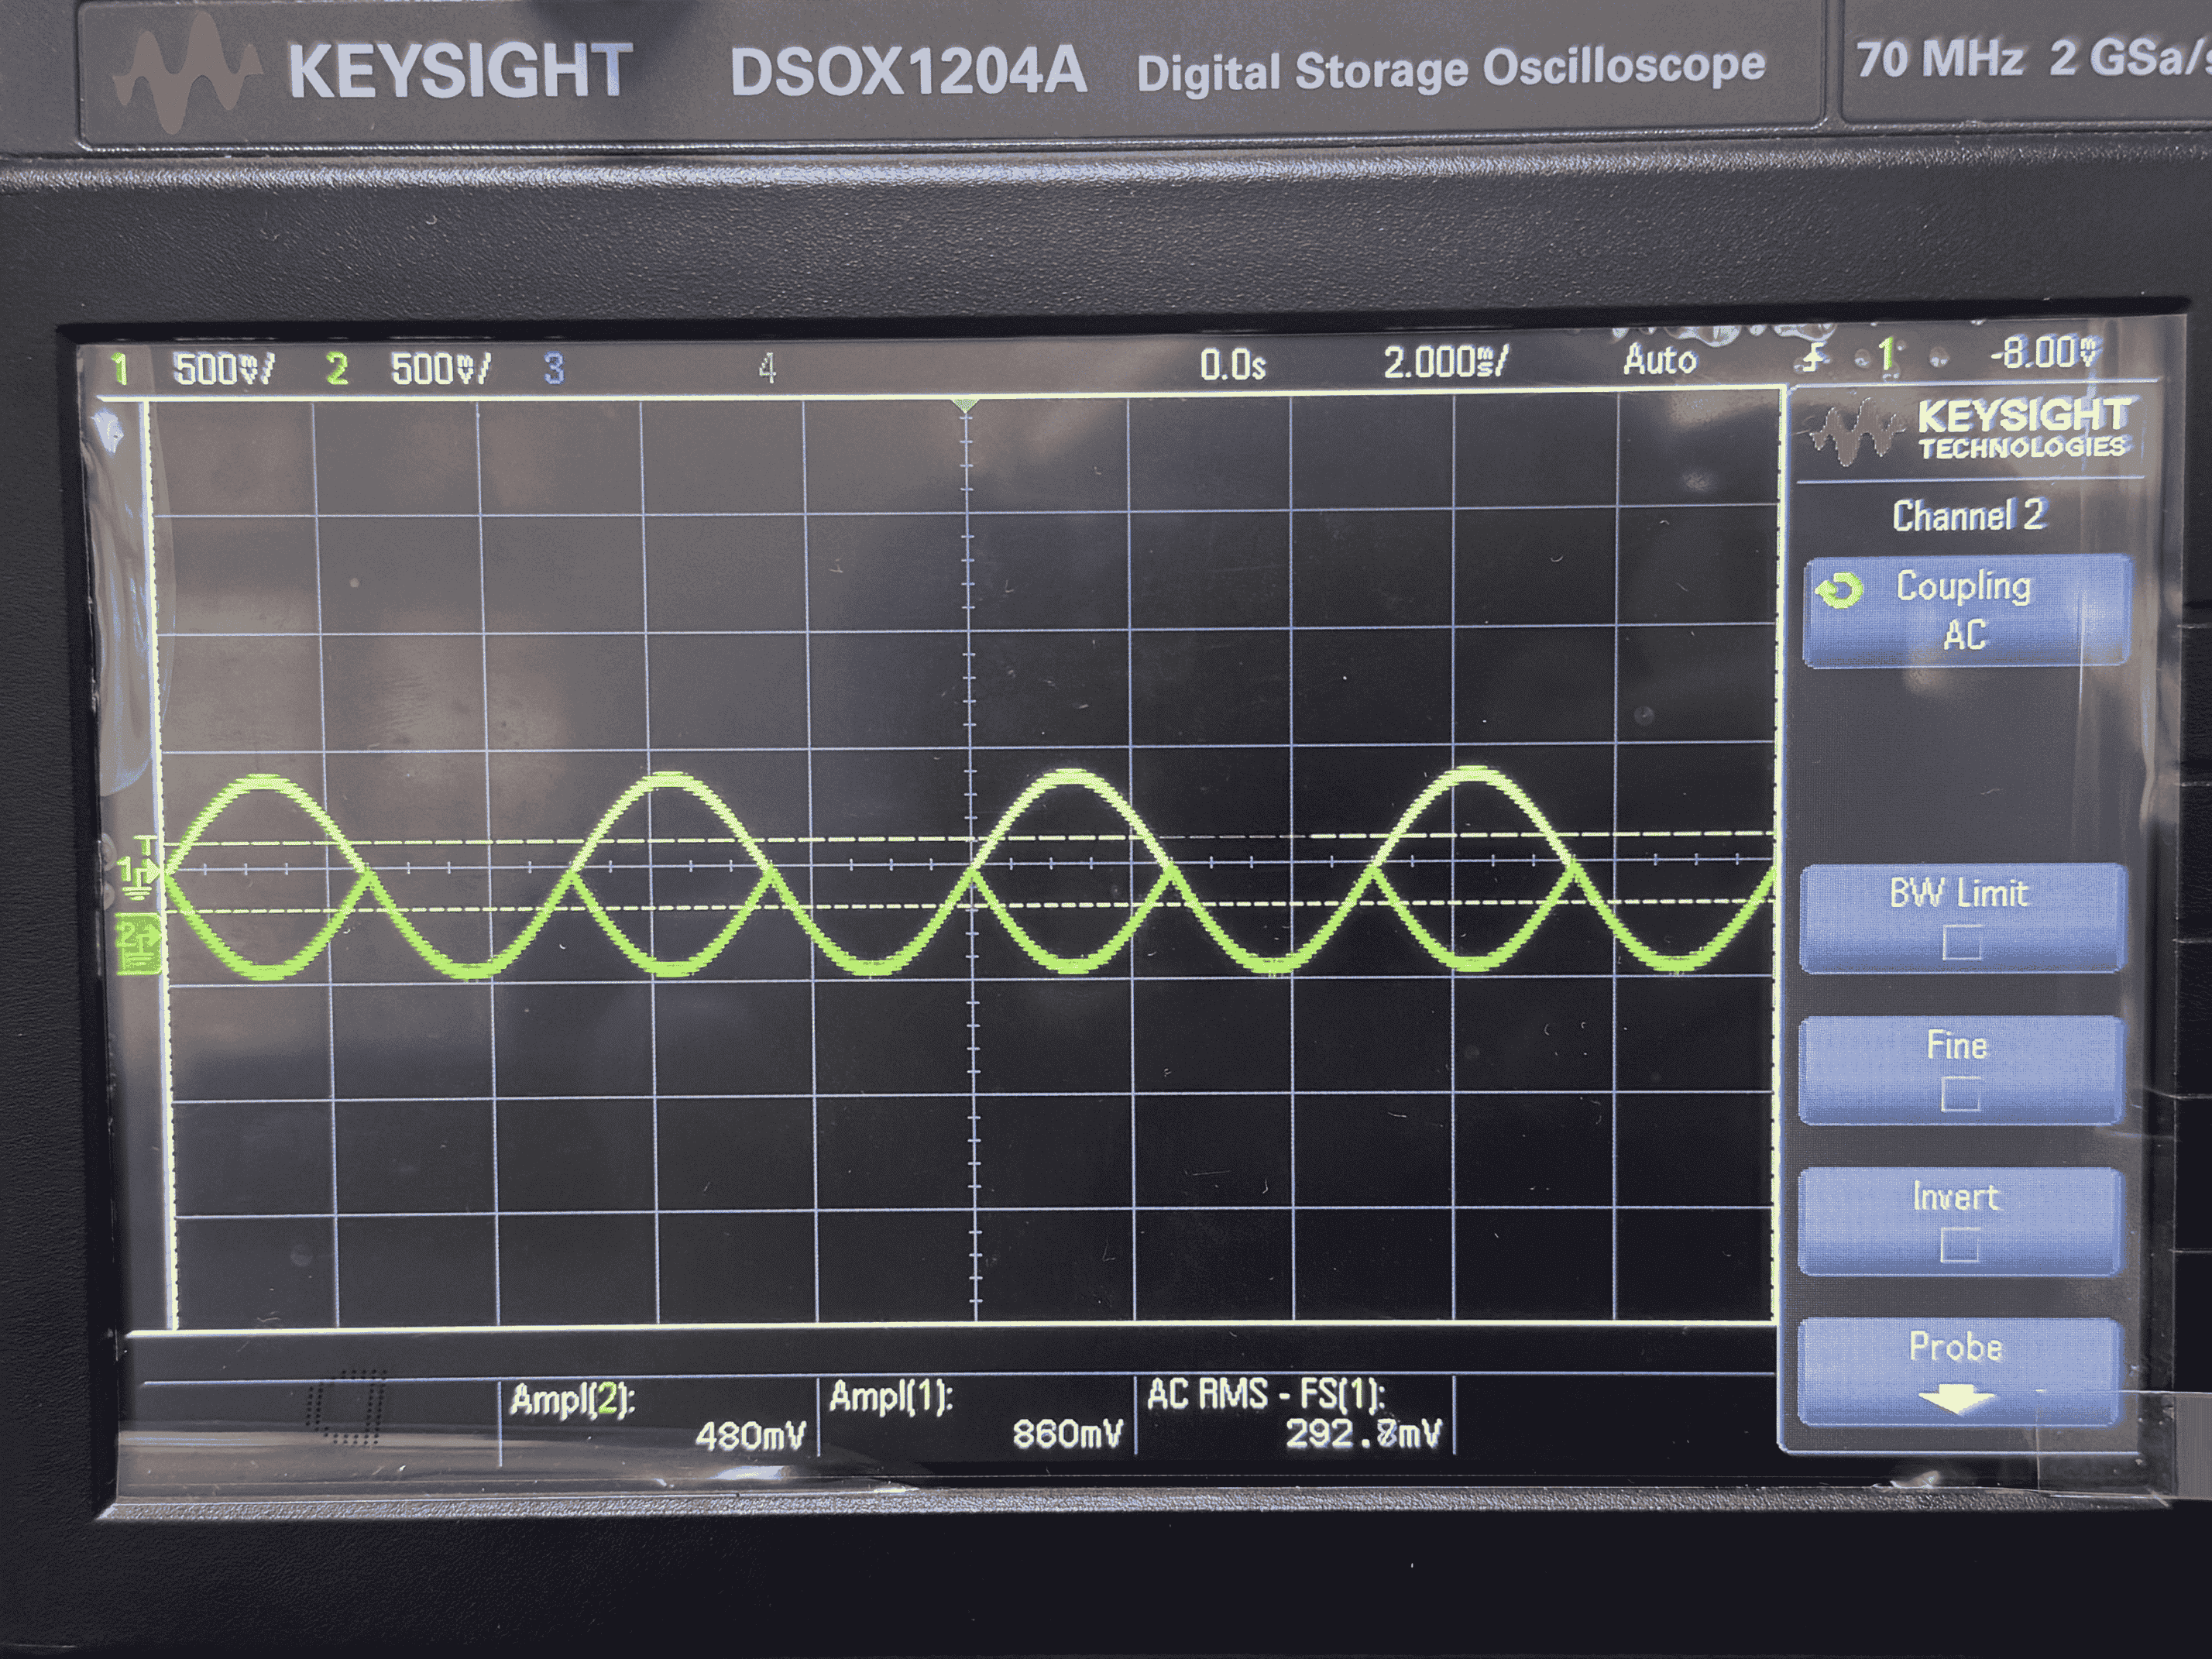
\includegraphics[width=1\linewidth]{Experiment_13/Images/13_4v.jpg}
            \caption{Amplitude $v_i=4V$}
            \label{wave:13-AC4}
        \end{subfigure}
        \begin{subfigure}{0.3\linewidth}
            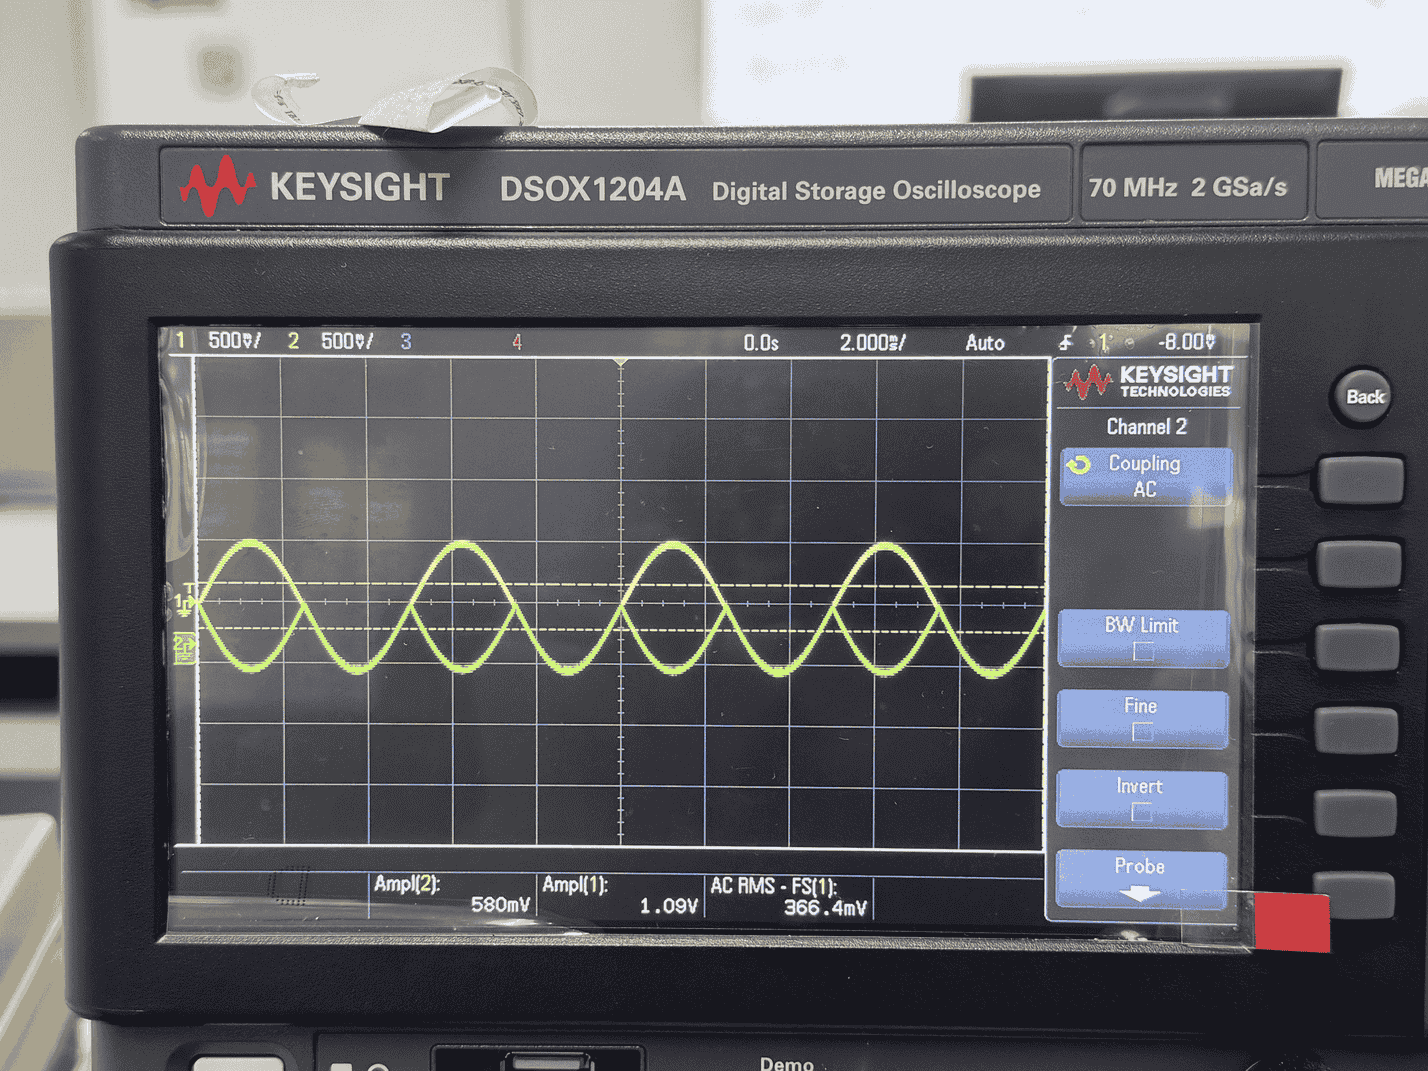
\includegraphics[width=1\linewidth]{Experiment_13/Images/13_5v.jpg}
            \caption{Amplitude $v_i=5V$}
            \label{wave:13-AC5}
        \end{subfigure}

        \caption{Observed Waveform of $V_i$ with input sinusoidal signal with a frequency 200 Hz}
    \end{figure}
    \FloatBarrier

    \subsubsection{DC Analysis}
    \begin{enumerate}[I]
        \item \textbf{Data Recorded}\newline
            For DC analysis, we change the input into a DC signal source, and vary the voltage $V_i$ from -12V to 12V, and record the output voltage $V_o$ and the voltage of each node $V_1$ to $V_5$. The recorded data is shown in the following table:
            \begin{table}[H]
                \centering
                \begin{tabular}{l|rrrrrr}
                    \toprule
                    $V_i$   & -12   & -5    & -1    & 1     & 5     & 12 \\
                    \midrule
                    $V_1$   & -2.002 & 0     & 0     & 0     & 0     & 0 \\
                    $V_2$   & 0     & 0     & 0     & 0     & 0     & 0 \\
                    $V_3$   & 8.556 & 5.557 & 1.518 & -0.4965 & -0.5766 & -0.6254 \\
                    $V_4$   & 7.913 & 4.953 & 0.9984 & -0.0011 & 0     & 0.4754 \\
                    $V_5$   & -0.002 & -0.002 & -0.002 & -0.0018 & -0.0015 & 0.9517 \\
                    $V_o$   & -4.143 & -5.131 & -1.029 & -1.013 & -5.045 & -9.211 \\
                    \bottomrule
                    \end{tabular}%                    
                \caption{Node voltage for Full-Wave Rectifier Circuit I}
                \label{tab:}
            \end{table}
        %\item \textbf{Data Analysis}\newline
    \end{enumerate}
    
\subsection{Experiment Conclusion}
    \subsubsection{Conclusion}
    In this experiment, we constructed one a full-wave rectifier circuit using two op-amps. We observed the output waveform with different input amplitude and frequency, and the output shows a full-wave rectified signal, with no signal loss. We also recorded the voltage of important nodes and the output voltage with different input voltage in the table.